\section{Ranking queries}

Ranking queries, also known as top-$k$ queries, focus on retrieving the $k$ best answers from a potentially extensive result set based on the concept of relevance.

The algorithm takes as inputs the cardinality $k$, the dataset $R$, and the scoring function $S$, with the output being the top $k$ tuples with the highest scores according to $S$.
The algorithm's approach involves computing scores for all tuples, sorting them based on these scores, and finally returning the top $k$ tuples.

However, this straightforward method becomes expensive for large datasets, especially when multiple relations are involved, necessitating the sorting of significant amounts of data.
Two crucial abilities are required: 
\begin{itemize}
    \item Ordering the tuples according to their scores with \texttt{ORDER BY}.
    \item Limiting the output cardinality to $k$ tuples with \texttt{FETCH FIRST k ROWS ONLY}.
\end{itemize} 
\begin{example}
    Consider the following queries: 
    \begin{lstlisting}[style=SQL]
-- Query one
SELECT *
FROM UsedCarsTable
WHERE Vehicle = 'Audi/A4'
AND Price <= 21000
ORDER BY 0.8*Price+0.2*Miles
-- Query two
SELECT *
FROM UsedCarsTable
WHERE Vehicle = 'Audi/A4'
ORDER BY 0.8*Price+0.2*Miles
    \end{lstlisting}
    Here, the values 0.8 and 0.2, termed weights, normalize preferences on price and mileage.
    The first query might miss relevant answers (near-miss), could result in information overload by returning all Audi A4 cars in the dataset.
\end{example}
Only the initial $k$ tuples are included in the result. 
If multiple sets of $k$ tuples meet the ordering directive, any of these sets is considered a valid answer, demonstrating non-deterministic semantics.

The evaluation of a top-$k$ query considers two basic aspects: query type (one relation, many relations, and aggregate results) and access paths (no index, indexes on all/some ranking attributes).
In the simplest case, in a top-$k$ selection query with a single relation, if the input is sorted according to $S$, only the first $k$ tuples need to be read.
If the tuples are not sorted, an in-memory sort is performed with a complexity of $O(N\log{k})$.
\begin{example}
    Consider the two-dimensional attribute space (Price, Mileage) illustrated in the previous example:
    \begin{figure}[H]
        \centering
        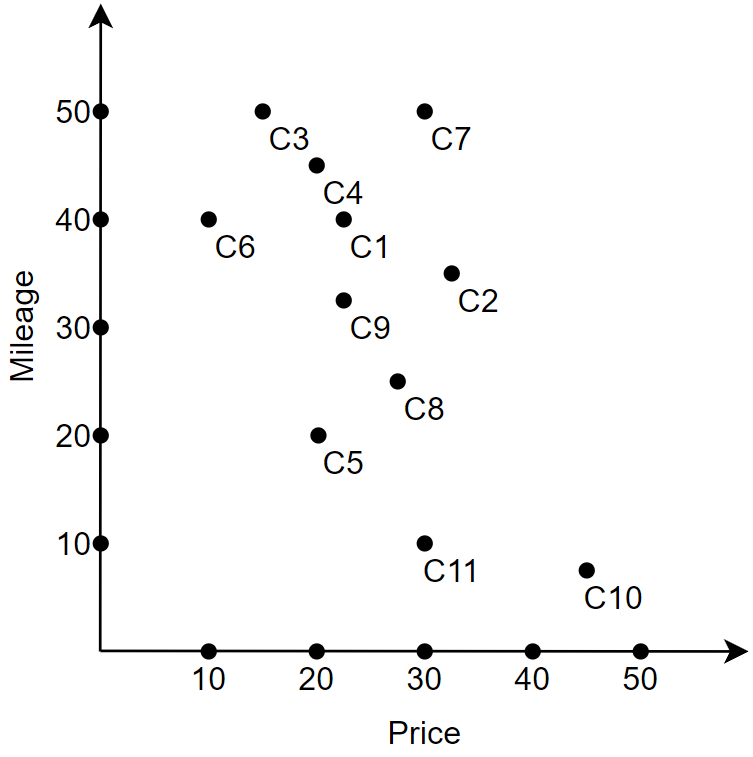
\includegraphics[width=0.25\linewidth]{images/ex1.png}
    \end{figure}
    In this representation, each tuple corresponds to a two-dimensional point $(p, m)$, where $p$ denotes the Price, and $m$ represents the Mileage. 
    The intuition behind minimizing $0.8 \cdot \text{Price} + 0.2 \cdot \text{Mileage}$ is the same as searching for points in proximity to $(0,0)$.
    Our preferences play a crucial role in determining the outcome. 
    Consider the equation of the line:
    \[0.8\cdot Price + 0.2\cdot Mileage = v\]
    Here, $v$ is a constant. 
    This equation can be alternatively expressed as:
    \[Mileage = -4\cdot Price + 5\cdot v\]
    From the previous equation we see that all the lines have a slope $-4$. 
    By definition, all points on the same line are equally good. 
    Modifying the weights may lead to variations in the optimal choice. 
    Importantly, the target of a query is not confined to $(0,0)$; it can be any point $q=(q_1,q_2)$.
\end{example}

In a general context, to assess the quality of a tuple $t$, we calculate its distance from the target point $q$. 
The desirability increases as the distance from $q$ decreases. 
When examining the distances, the model can be characterized by the following components:
\begin{itemize}
    \item An $m$-dimensional space $A = (A_1, A_2, \dots, A_m)$ comprising ranking attributes, where $m \geq 1$.
    \item A relation $R(A_1, A_2, \dots, B_1, B_2, \dots)$, with $B_1, B_2, \dots$ representing additional attributes.
    \item A target point $q = (q_1, q_2, \dots, q_m)$ located in $A$.
    \item A distance function $d: A \times A \rightarrow \mathbb{R}^{+}$, quantifying the distance between points in $A$.
\end{itemize}
\begin{definition}
    The top-$k$ query is called $k$-\emph{nearest neighbors} if given a point $q$, a relation $R$, an integer $k \geq 1$, and a distance function $d$ it determines the $k$ tuples in $R$ that are closest to $q$ according to $d$. 

    The distance function, denoted as $L_p$-\emph{norms}, is defined by the formula:
    \[L_p(t,q)=\left(\sum_{i=1}^{m}{\left\lvert t_i-q_i \right\rvert^{p}}\right)^{\frac{1}{p}}\]
\end{definition}

\paragraph*{Distance functions}
Significant instances of the $L_p$-norm include:
\begin{itemize}
    \item Euclidean distance (ellipsoids): $L_2(t,q)=\sqrt{\sum_{i=1}^{m}{\left\lvert t_i-q_i \right\rvert^{2}}}$
    \item Manhattan distance (rhomboids): $L_1(t,q)=\sum_{i=1}^{m}{\left\lvert t_i-q_i \right\rvert}$
    \item Čebyšëv distance (rectangles): $L_{\infty}(t,q)=\max_{i}\{\left\lvert t_i-q_i\right\rvert\}$
\end{itemize}
The shape of the attribute space depends on the distance function and the weight associated to each coordinate: 
\begin{itemize}
    \item Euclidean distance (hyper-ellipsoids):
        \[L_2(t,q;W)=\sqrt{\sum_{i=1}^{m}{w_i\left\lvert t_i-q_i \right\rvert^{2}}}\]
    \item Manhattan distance (hyper-rhomboids): 
        \[L_1(t,q;W)=\sum_{i=1}^{m}{w_i\left\lvert t_i-q_i \right\rvert}\]
    \item Čebyšëv distance (hyper-rectangles): 
        \[L_{\infty}(t,q;W)=\max_{i}\{w_i \left\lvert t_i-q_i\right\rvert\}\]
\end{itemize}

\paragraph*{Top-k join query}
In a top-$k$ join query with $n>1$ input relations and a scoring function $S$ defined on the result of the join, the general formulation is as follows:
\begin{lstlisting}[style=SQL]
SELECT <attributes>
FROM R1,R2,...,Rn
WHERE <conditions>
ORDER BY S(p1,p2,...,pm) [DESC]
FETCH FIRST k ROWS ONLY             
\end{lstlisting}
In this query, $p_1, p_2, \dots, p_m$ represent the scoring criteria.

In top-$k$ $1-1$ join queries, where all joins are on a common key attribute, two main scenarios are possible:
\begin{itemize}
    \item There is an index for retrieving tuples according to each preference.
    \item The relation is spread over several sites, each providing information only on part of the objects.
\end{itemize}
We make the following assumptions: 
\begin{itemize}
    \item Each input list supports sorted access, returning the identifier of the next best object and its partial score $p_j$.
    \item Each input list supports random access, returning the partial score of an object given its identifier.
    \item The identifier of an object is the same across all inputs.
    \item Each input consists of the same set of objects.
\end{itemize}
\begin{example}
    Given reviews on two different sites:
    \begin{table}[H]
        \centering
        \begin{tabular}{ccccc}
        \multicolumn{1}{l}{\textbf{EatWell}}     &                                     & $\:\:\:\:\:\:$                 & \multicolumn{1}{l}{\textbf{BreadAndWine}} &                                  \\ \cline{1-2} \cline{4-5} 
        \multicolumn{1}{|l}{\textbf{Name}}       & \multicolumn{1}{c|}{\textbf{Score}} & \multicolumn{1}{c|}{\textbf{}} & \multicolumn{1}{l}{\textbf{Name}}        & \multicolumn{1}{c|}{\textbf{Score}} \\ \cline{1-2} \cline{4-5} 
        \multicolumn{1}{|l}{The old mill}        & \multicolumn{1}{c|}{9.2}            & \multicolumn{1}{c|}{}          & \multicolumn{1}{l}{Da Gino}              & \multicolumn{1}{c|}{9.0}            \\
        \multicolumn{1}{|l}{The canteen}         & \multicolumn{1}{c|}{9.0}            & \multicolumn{1}{c|}{}          & \multicolumn{1}{l}{Cheers!}              & \multicolumn{1}{c|}{8.5}            \\  
        \multicolumn{1}{|l}{Cheers!}             & \multicolumn{1}{c|}{8.3}            & \multicolumn{1}{c|}{}          & \multicolumn{1}{l}{The old mill}         & \multicolumn{1}{c|}{7.5}            \\ 
        \multicolumn{1}{|l}{Da Gino}             & \multicolumn{1}{c|}{7.5}            & \multicolumn{1}{c|}{}          & \multicolumn{1}{l}{Chez Paul}            & \multicolumn{1}{c|}{7.5}            \\ 
        \multicolumn{1}{|l}{Let's eat!}          & \multicolumn{1}{c|}{6.4}            & \multicolumn{1}{c|}{}          & \multicolumn{1}{l}{The canteen}          & \multicolumn{1}{c|}{7.0}            \\ 
        \multicolumn{1}{|l}{Chez Paul}           & \multicolumn{1}{c|}{5.5}            & \multicolumn{1}{c|}{}          & \multicolumn{1}{l}{Los pollos hermanos}  & \multicolumn{1}{c|}{6.5}            \\ 
        \multicolumn{1}{|l}{Los pollos hermanos} & \multicolumn{1}{c|}{5.0}            & \multicolumn{1}{c|}{}          & \multicolumn{1}{l}{Let's eat!}           & \multicolumn{1}{c|}{6.0}            \\ \cline{1-2} \cline{4-5} 
        \end{tabular}
    \end{table}
    If we aggregate the two tables with the following query:
    \begin{lstlisting}[style=SQL]
SELECT *
FROM EatWell EW, BreadAndWine BW
WHERE EW.Name = BW.Name
ORDER BY EW.Score + BW.Score DESC
FETCH FIRST 1 ROW ONLY 
    \end{lstlisting}
    The result would be:
    \begin{table}[H]
        \centering
        \begin{tabular}{|lc|}
        \hline
        \textbf{Name}       & \textbf{Global score} \\ \hline
        Cheers!             & 16.8                  \\ \hline
        The old mill        & 16.7                  \\ \hline
        Da Gino             & 16.5                  \\ \hline
        The canteen         & 16.0                  \\ \hline
        Chez Paul           & 13.0                  \\ \hline
        Let's eat!          & 12.4                  \\ \hline
        Los pollos hermanos & 11.5                  \\ \hline
        \end{tabular}
    \end{table}
    Note that the winner is not the best locally.
\end{example}

\paragraph*{Score space}
Each object $o$ returned by the input $L_j$ has an associated local/partial score $p_j(o) \in [0,1]$. 
Scores are normalized, and the hypercube $[0,1]^m$ is called the score space.
The point $p(o) = (p_1(o), p_2(o), \dots, p_m(o)) \in [0,1]^m$ is the map of $o$ into the score space. 
The global score $S(o)$ of $o$ is computed using a scoring function $S$ that combines the local scores of $o$:
\[S(o) \equiv  S(p(o)) = S(p_1(o),p_2(o),\dots,p_m(o))\]
With $S:[0,1]^m \rightarrow \mathbb{R}^{+}$. 
\begin{example}
    Consider the attribute space $A = (Price,Mileage)$
    \begin{figure}[H]
        \centering
        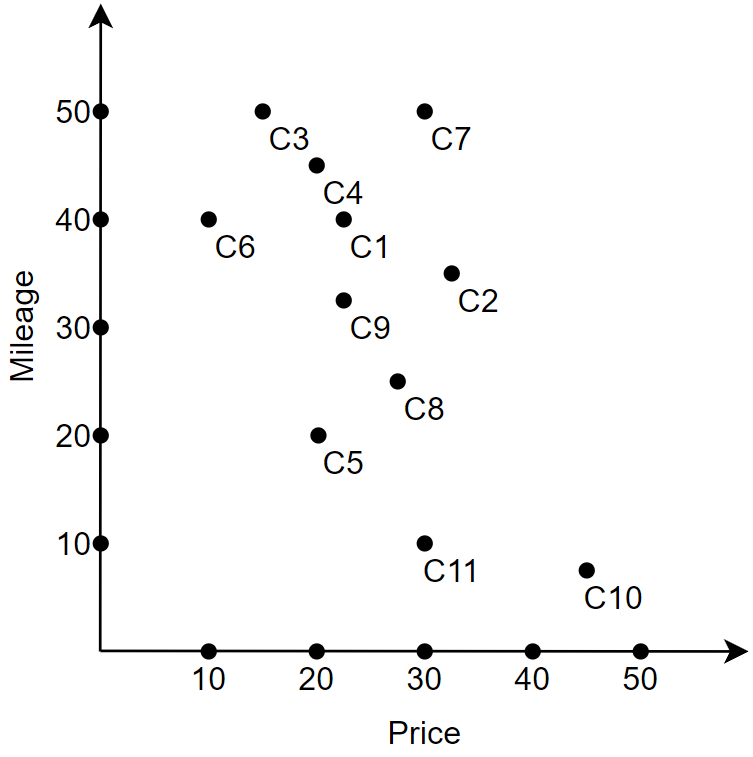
\includegraphics[width=0.25\linewidth]{images/ex1.png}
    \end{figure}
    If we choose $MaxP = 50,000$ and $MaxM = 80,000$, a generic point $o$ is mapped with these formulas:
    \[p_1(o) = 1 - \dfrac{o.Price}{MaxP}\]
    \[p_2(o) = 1 - \dfrac{o.Mileage}{MaxM}\]
    The new graph is as follows: 
    \begin{figure}[H]
        \centering
        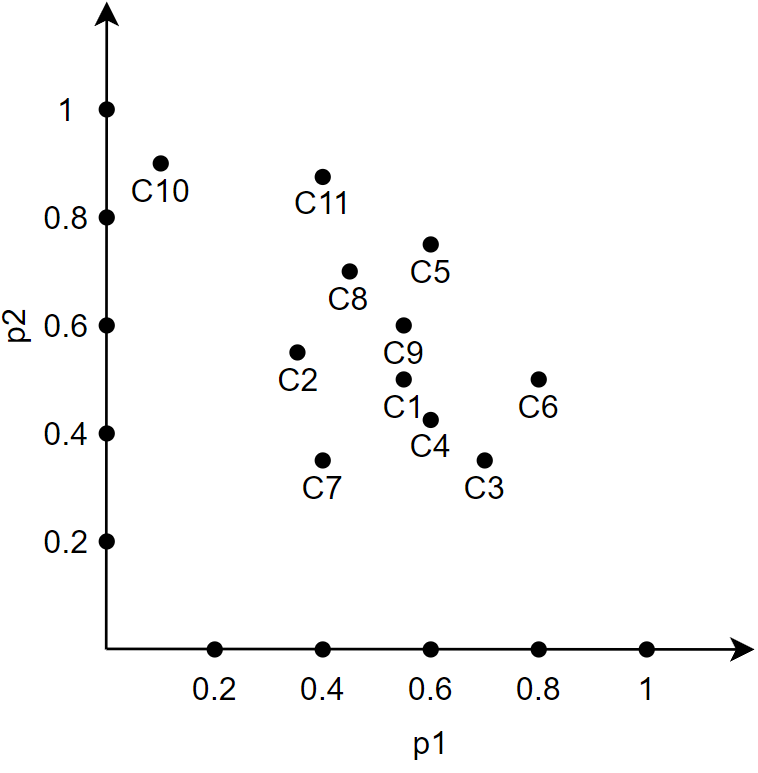
\includegraphics[width=0.3\linewidth]{images/ex2.png}
    \end{figure}
\end{example}

\paragraph*{Scoring functions}
The most common scoring functions are: 
\begin{itemize}
    \item Average, that weighs preferences equally: 
        \[\textnormal{SUM}(o) \equiv \textnormal{SUM}(p(o)) = p_1(o) + p_2(o) + \dots + p_m(o)\]
    \item Weighted sum, that weighs the preferences differently:
        \[\textnormal{WSUM}(o) \equiv \textnormal{WSUM}(p(o)) = w_1p_1(o) + w_2p_2(o) + \dots + w_mp_m(o)\]
    \item Minimum, that considers the worst partial score: 
        \[\textnormal{MIN}(o) \equiv \textnormal{MIN}(p(o)) = \min\{p_1(o),p_2(o),\dots, p_m(o)\}\]
    \item Maximum, that considers the best partial score: 
        \[\textnormal{MAX}(o) \equiv \textnormal{MAX}(p(o)) = \max\{p_1(o),p_2(o),\dots, p_m(o)\}\]       
\end{itemize}
Even with the minimum scoring function, the goal is to retrieve the $k$ objects with the highest global scores.

\paragraph*{Iso-score curves}
Iso-score curves in the score space can be defined, representing sets of points with the same global score.
\begin{example}
    In the previous graph we have that the iso-score curves for the maximum function are: 
    \begin{figure}[H]
        \centering
        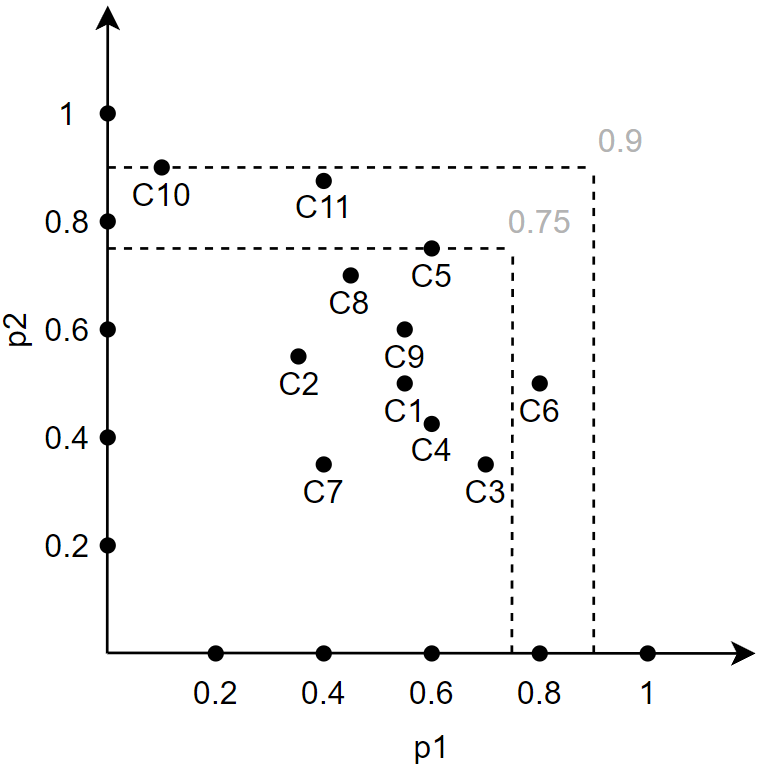
\includegraphics[width=0.3\linewidth]{images/iso.png}
    \end{figure}
    In the previous graph we have that the iso-score curves for the minimum function are: 
    \begin{figure}[H]
        \centering
        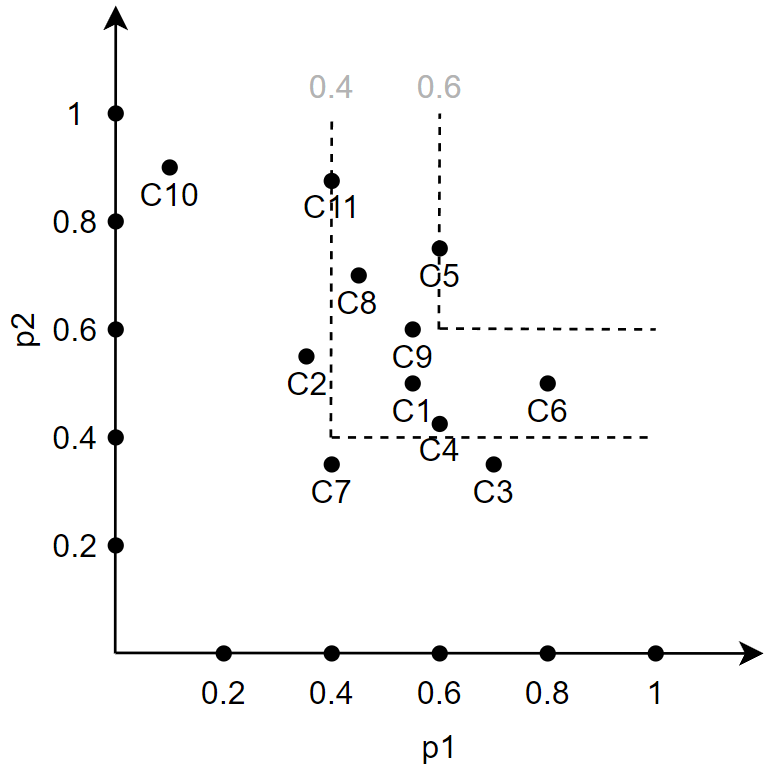
\includegraphics[width=0.3\linewidth]{images/isomin.png}
    \end{figure}
\end{example}

\subsection{B-zero algorithm}
Efficient computation of the result of a top-k 1-1 join query using a maximum scoring function $S$ can be achieved through the $B_0$ algorithm. 
The inputs for this algorithm are an integer $k \geq 1$ and a ranked list $R_1,\dots,R_m$.
The algorithm proceeds as follows:
\begin{enumerate}
    \item Perform $k$ sorted accesses on each list and store objects and partial scores in a buffer $B$. 
    \item For each object in $B$, compute the maximum of its (available) partial scores.
    \item Return the top $k$ objects with maximum score.
\end{enumerate}
\begin{property}
    $B_0$ algorithm is instance-optimal. 
\end{property}
\begin{example}
    For instance, given reviews on two different sites:
    \begin{table}[H]
        \centering
        \begin{tabular}{ccccc}
        \multicolumn{1}{l}{\textbf{EatWell}}     &                                     & $\:\:\:\:\:\:$                 & \multicolumn{1}{l}{\textbf{BreadAndWine}} &                                  \\ \cline{1-2} \cline{4-5} 
        \multicolumn{1}{|l}{\textbf{Name}}       & \multicolumn{1}{c|}{\textbf{Score}} & \multicolumn{1}{c|}{\textbf{}} & \multicolumn{1}{l}{\textbf{Name}}        & \multicolumn{1}{c|}{\textbf{Score}} \\ \cline{1-2} \cline{4-5} 
        \multicolumn{1}{|l}{The old mill}        & \multicolumn{1}{c|}{9.2}            & \multicolumn{1}{c|}{}          & \multicolumn{1}{l}{Da Gino}              & \multicolumn{1}{c|}{9.0}            \\
        \multicolumn{1}{|l}{The canteen}         & \multicolumn{1}{c|}{9.0}            & \multicolumn{1}{c|}{}          & \multicolumn{1}{l}{Cheers!}              & \multicolumn{1}{c|}{8.5}            \\  
        \multicolumn{1}{|l}{Cheers!}             & \multicolumn{1}{c|}{8.3}            & \multicolumn{1}{c|}{}          & \multicolumn{1}{l}{The old mill}         & \multicolumn{1}{c|}{7.5}            \\ 
        \multicolumn{1}{|l}{Da Gino}             & \multicolumn{1}{c|}{7.5}            & \multicolumn{1}{c|}{}          & \multicolumn{1}{l}{Chez Paul}            & \multicolumn{1}{c|}{7.5}            \\ 
        \multicolumn{1}{|l}{Let's eat!}          & \multicolumn{1}{c|}{6.4}            & \multicolumn{1}{c|}{}          & \multicolumn{1}{l}{The canteen}          & \multicolumn{1}{c|}{7.0}            \\ 
        \multicolumn{1}{|l}{Chez Paul}           & \multicolumn{1}{c|}{5.5}            & \multicolumn{1}{c|}{}          & \multicolumn{1}{l}{Los pollos hermanos}  & \multicolumn{1}{c|}{6.5}            \\ 
        \multicolumn{1}{|l}{Los pollos hermanos} & \multicolumn{1}{c|}{5.0}            & \multicolumn{1}{c|}{}          & \multicolumn{1}{l}{Let's eat!}           & \multicolumn{1}{c|}{6.0}            \\ \cline{1-2} \cline{4-5} 
        \end{tabular}
    \end{table}
    If we apply the $B_0$ algorithm with $k=3$, selecting the first three rows from both tables (which are sorted), and summing all the values by identifier, we obtain the final rank with the maximum value:
    \begin{table}[H]
        \centering
        \begin{tabular}{|lc|}
        \hline
        \textbf{Name} & \textbf{S} \\ \hline
        The old mill  & 9.2        \\ 
        Da Gino       & 9.0        \\ 
        The canteen   & 9.0        \\ 
        Cheers!       & 8.5        \\ \hline
        \end{tabular}
    \end{table}
\end{example}

\subsection{A-zero algorithm}
The A-zero algorithm, also known as Fagin's algorithm, is applicable to every monotonic scoring function. 
The algorithm takes an integer $k$ and a monotone function $S$ combining ranked lists $R_1,\dots,R_m$ as inputs, producing the top $k$ (object-score) tuples as output.
The algorithm follows these steps:
\begin{enumerate}
    \item Extract the same number of objects through sorted accesses in each list until there are at least $k$ common objects.
    \item For each extracted object, compute its overall score by making random accesses wherever needed.
    \item Among these, output the $k$ objects with the best overall score. 
\end{enumerate}
The complexity of this algorithm is $O(N^{\frac{m-1}{m}}k^{\frac{1}{m}})$, which is sublinear in the number $N$ of objects. 
The stopping criterion is independent of the scoring function, and it is not instance-optimal.
\begin{example}
    Consider hotel reviews on different sites:
    \begin{table}[H]
        \centering
        \begin{tabular}{|lc|c|lc|}
        \cline{1-2} \cline{4-5}
        \textbf{Name} & \textbf{Cheapness} & $\:\:\:\:\:\:$ & \textbf{Name} & \textbf{Rating} \\ \cline{1-2} \cline{4-5} 
        Ibis          & 0.92               &                & Crillon       & 0.9             \\ 
        Etap          & 0.91               &                & Novotel       & 0.9             \\  
        Novotel       & 0.85               &                & Sheraton      & 0.8             \\  
        Mercure       & 0.85               &                & Hilton        & 0.7             \\  
        Hilton        & 0.825              &                & Ibis          & 0.7             \\  
        Sheraton      & 0.8                &                & Ritz          & 0.7             \\  
        Crillon       & 0.75               &                & Lutetia       & 0.6             \\  
        $\dots$       & $\dots$            &                & $\dots$       & $\dots$         \\ \cline{1-2} \cline{4-5} 
        \end{tabular}
    \end{table}
    Using the scoring function $0.5 \cdot \text{cheapness} + 0.5 \cdot \text{rating}$ and $k=2$, iterate on the rows until $k$ hotels are found in all columns (in this case, Ibis, Novotel, and Hilton). 
    Complete the score of the remaining incomplete hotels by making random accesses to find the missing values. 
    After summing up the information, compute the final ranking with the given score function, resulting in:
    \begin{table}[H]
        \centering
        \begin{tabular}{|lc|}
        \hline
        \textbf{Top $\boldsymbol{k}$} & \textbf{Score} \\ \hline
        Novotel                       & 0.875          \\ 
        Crillon                       & 0.825          \\ \hline
        \end{tabular}
    \end{table}
\end{example}
The primary limitation of this algorithm lies in its dependence on accesses, leading to an underutilization of the specificity inherent in certain scoring functions. 
Additionally, the memory requirements have the potential to become impractical.
While there are possibilities for improvements, substantial enhancements in complexity can only be achieved by modifying the stopping condition.

\subsection{Threshold algorithm}
The threshold algorithm takes as inputs an integer $k$ and a monotone function $S$ that combines ranked lists $R_1,\dots,R_m$. 
It outputs the top $k$ (object, score) tuples. 
The algorithm follows these steps:
\begin{enumerate}
    \item Perform sorted access in parallel in each list $R_i$. 
    \item For each object $o$, conduct random accesses in the other lists $R_j$ to extract score $s_j$. 
    \item Compute the overall score $S(s_1, \dots, s_m)$. 
        If the value is among the $k$ highest seen so far, and remember $o$. 
    \item Let $s_{L_i}$ be the last score seen under sorted access for $R_i$. 
    \item Define the threshold $T=S(s_{L_1}, \dots, s_{L_m})$. 
    \item If the score of the $k$-th object is worse than $T$, go to step one. 
    \item Return the current top$k$ objects. 
\end{enumerate}
\begin{property}
    The threshold algorithm is instance optimal among all algorithms that use random and sorted accesses. 
\end{property}
The stopping criterion depends on the function and not on the number of accesses. 
\begin{example}
    Consider hotel reviews with cheapness and rating values.
    \begin{table}[H]
        \centering
        \begin{tabular}{|lc|c|lc|}
        \cline{1-2} \cline{4-5}
        \textbf{Name} & \textbf{Cheapness} & $\:\:\:\:\:\:$ & \textbf{Name} & \textbf{Rating} \\ \cline{1-2} \cline{4-5} 
        Ibis          & 0.92               &                & Crillon       & 0.9             \\ 
        Etap          & 0.91               &                & Novotel       & 0.9             \\ 
        Novotel       & 0.85               &                & Sheraton      & 0.8             \\ 
        Mercure       & 0.85               &                & Hilton        & 0.7             \\ 
        Hilton        & 0.825              &                & Ibis          & 0.7             \\ 
        Sheraton      & 0.8                &                & Ritz          & 0.7             \\ 
        Crillon       & 0.75               &                & Lutetia       & 0.6             \\ 
        $\dots$       & $\dots$            &                & $\dots$       & $\dots$         \\ \cline{1-2} \cline{4-5} 
        \end{tabular}
    \end{table}
    The scoring function is $0.5 \cdot cheapness+0.5 \cdot rating$, and $k=2$. 
    We do a sorted access, and we put the hotels in the first row in the buffer with the mean value of both variables (the second can be found with a random access). 
    The threshold point is $(0.92,0.9)$ and has a value of $0.91$, found with the scoring function. 
    We continue to do this procedure, and we update the top $k$ hotels only if the found hotel has a better score of at least one of the hotels in the buffer (note that we keep in the buffer only the top $k$ hotels, while we delete the others). 
    We stop the iteration when the value of all the objects in the buffer is greater or equal to the threshold value. 
    In this example this happens after three iteration. 
    The buffer contains the top $k$ hotels with their corresponding scores.
    \begin{table}[H]
        \centering
        \begin{tabular}{|lc|}
        \hline
        \textbf{Top $\boldsymbol{k}$} & \textbf{Score} \\ \hline
        Novotel                       & 0.875          \\ 
        Crillon                       & 0.825          \\ \hline
        \end{tabular}
    \end{table}
    The threshold point has a value of $0.825$
\end{example}
In general, the Threshold Algorithm outperforms the Fagin Algorithm since it can adapt to the specific scoring function. 
To assess the performance of Threshold Algorithm, we evaluate the middleware cost using the following formula:
\[\textnormal{cost} = SA \cdot c_{SA} + RA \cdot c_{RA}\]
Where:
\begin{itemize}
    \item $SA$ is the total number of sorted accesses.
    \item $RA$ is the total number of random accesses.
    \item $c_{SA}$ is the base cost of sorted accesses.
    \item $c_{RA}$ is the base cost of random accesses.
\end{itemize}

\subsection{No Random Access algorithm}
The No Random Access algorithm returns the top-$k$ objects, but their scores might be uncertain. 
The fundamental idea behind this algorithm is to maintain, for each selected object $o$, both a lower bound and an upper bound on its score.
Thus, an unlimited buffer is required to store the objects, sorted by decreasing lower bound values.
The algorithm stops when the upper bound of a new object is less than or equal to the worst lower bound among the best objects.
The inputs include an integer $k \geq 1$, a monotone function $S$ combining ranked lists $R_1, \dots, R_m$, and the output is the ranking without the scores of the objects. 
The procedure is as follows:
\begin{enumerate}
    \item Perform a sorted access to each list.
    \item Store each retrieved object $o$ in buffer $B$, maintaining $S^{-}(o)$ and $S^{+}(o)$ along with a threshold $\tau$.
    \item Repeat from step one as long as:
        \[S^{-}(B[k])<\max\{\max\{S^{+}(B[i]),i>k\},S(\tau)\}\]
\end{enumerate}
\begin{example}
    Given tables based on three different criteria:
    \begin{table}[H]
        \centering
        \begin{tabular}{cccccccc}
        \multicolumn{1}{l}{$R_1$}                 & \multicolumn{1}{l}{}                & \multicolumn{1}{l}{$\:\:\:\:\:\:$} & \multicolumn{1}{l}{$R_2$}                & \multicolumn{1}{l}{}                & \multicolumn{1}{l}{$\:\:\:\:\:\:$} & \multicolumn{1}{l}{$R_3$}                & \multicolumn{1}{l}{}                \\ \cline{1-2} \cline{4-5} \cline{7-8} 
        \multicolumn{1}{|c}{\textbf{ID}} & \multicolumn{1}{c|}{\textbf{Score}} & \multicolumn{1}{c|}{\textbf{}}     & \multicolumn{1}{c}{\textbf{ID}} & \multicolumn{1}{c|}{\textbf{Score}} & \multicolumn{1}{c|}{\textbf{}}     & \multicolumn{1}{c}{\textbf{ID}} & \multicolumn{1}{c|}{\textbf{Score}} \\ \cline{1-2} \cline{4-5} \cline{7-8} 
        \multicolumn{1}{|c}{$o_1$}               & \multicolumn{1}{c|}{1.0}            & \multicolumn{1}{c|}{}              & \multicolumn{1}{c}{$o_2$}               & \multicolumn{1}{c|}{0.8}            & \multicolumn{1}{c|}{}              & \multicolumn{1}{c}{$o_7$}               & \multicolumn{1}{c|}{0.6}            \\  
        \multicolumn{1}{|c}{$o_7$}               & \multicolumn{1}{c|}{0.9}            & \multicolumn{1}{c|}{}              & \multicolumn{1}{c}{$o_3$}               & \multicolumn{1}{c|}{0.75}           & \multicolumn{1}{c|}{}              & \multicolumn{1}{c}{$o_2$}               & \multicolumn{1}{c|}{0.6}            \\  
        \multicolumn{1}{|c}{$o_2$}               & \multicolumn{1}{c|}{0.7}            & \multicolumn{1}{c|}{}              & \multicolumn{1}{c}{$o_4$}               & \multicolumn{1}{c|}{0.5}            & \multicolumn{1}{c|}{}              & \multicolumn{1}{c}{$o_3$}               & \multicolumn{1}{c|}{0.5}            \\  
        \multicolumn{1}{|c}{$o_6$}               & \multicolumn{1}{c|}{0.2}            & \multicolumn{1}{c|}{}              & \multicolumn{1}{c}{$o_1$}               & \multicolumn{1}{c|}{0.4}            & \multicolumn{1}{c|}{}              & \multicolumn{1}{c}{$o_5$}               & \multicolumn{1}{c|}{0.1}            \\  
        \multicolumn{1}{|c}{$\dots$}             & \multicolumn{1}{c|}{$\dots$}        & \multicolumn{1}{c|}{}              & \multicolumn{1}{c}{$\dots$}             & \multicolumn{1}{c|}{$\dots$}        & \multicolumn{1}{c|}{}              & \multicolumn{1}{c}{$\dots$}             & \multicolumn{1}{c|}{$\dots$}        \\ \cline{1-2} \cline{4-5} \cline{7-8} 
        \end{tabular}
    \end{table}
    We decide to use sum as score function, and $k=2$. 
    For the first iteration we add to the buffer the  objects in the first row with a lower bound corresponding to the sum of the score of each object and the upper bound corresponding to the sum of all the object in the row. 
    The threshold is the sum of all the scores of the row: 
    \begin{table}[H]
        \centering
        \begin{tabular}{|ccc|}
        \hline
        \textbf{Identifier} & \textbf{Lower bound} & \textbf{Upper bound} \\ \hline
        $o_1$               & 1.0                  & 2.4                  \\ 
        $o_2$               & 0.8                  & 2.4                  \\ 
        $o_7$               & 0.6                  & 2.4                  \\ \hline
        \end{tabular}
    \end{table}
    The threshold has a value of $2.4$, and so we have that:
    \[0.8<\max\{2.4,2.4\}\]
    Since that the inequality is verified we have to do another iteration, that creates the following table: 
    \begin{table}[H]
        \centering
        \begin{tabular}{|ccc|}
        \hline
        \textbf{Identifier} & \textbf{Lower bound} & \textbf{Upper bound} \\ \hline
        $o_7$               & 1.5                  & 2.25                 \\ 
        $o_2$               & 1.4                  & 2.3                  \\ 
        $o_1$               & 1.0                  & 2.35                 \\ 
        $o_3$               & 0.75                 & 2.25                 \\ \hline
        \end{tabular}
    \end{table}
    The threshold has a value of $2.25$, and so we have that:
    \[1.4<\max\{2.35,2.25\}\]
    Since that the inequality is verified we have to do another iteration, that creates the following table: 
    \begin{table}[H]
        \centering
        \begin{tabular}{|ccc|}
        \hline
        \textbf{Identifier} & \textbf{Lower bound} & \textbf{Upper bound} \\ \hline
        $o_2$               & 2.1                  & 2.1                  \\ 
        $o_7$               & 1.5                  & 2.0                  \\ 
        $o_3$               & 1.25                 & 1.95                 \\
        $o_1$               & 1.0                  & 2.0                  \\ 
        $o_4$               & 0.5                  & 1.7                  \\ \hline
        \end{tabular}
    \end{table}
    The threshold has a value of $1.7$, and so we have that:
    \[1.5<\max\{2.0,1.7\}\]
    Since that the inequality is verified we have to do another iteration, that creates the following table: 
    \begin{table}[H]
        \centering
        \begin{tabular}{|ccc|}
        \hline
        \textbf{Identifier} & \textbf{Lower bound} & \textbf{Upper bound} \\ \hline
        $o_2$               & 2.1                  & 2.1                  \\ 
        $o_7$               & 1.5                  & 1.9                  \\ 
        $o_1$               & 1.4                  & 1.5                  \\ 
        $o_3$               & 1.25                 & 1.45                 \\ 
        $o_4$               & 0.5                  & 0.8                  \\ 
        $o_6$               & 0.2                  & 0.7                  \\ 
        $o_5$               & 0.1                  & 0.7                  \\ \hline
        \end{tabular}
    \end{table}
    The threshold has a value of $1.7$, and so we have that:
    \[1.5<\max\{1.5,0.7\}\]
    Since that the inequality is not verified the algorithm return the first two elements in the table. 
\end{example}
\begin{property}
    No Random Access algorithm is instance optimal among all algorithms that do not make random accesses.
\end{property}

\subsection{Summary}
\begin{table}[H]
    \centering
    \begin{tabular}{l|ccc}
    \multicolumn{1}{c|}{\textbf{Algorithm}} & \textbf{Scoring function} & \textbf{Data access} & \textbf{Notes}                       \\ \hline
    $B_0$                                   & MAX                       & sorted               & instance-optimal                     \\
    FA                                      & monotone                  & sorted and random    & cost independent of function         \\
    TA                                      & monotone                  & sorted and random    & instance-optimal                     \\
    NRA                                     & monotone                  & sorted               & instance-optimal, uncertain         
    \end{tabular}
\end{table}

The main aspects of the ranking queries are: 
\begin{itemize}
    \item Effectiveness in pinpointing the top objects based on a designated scoring function.
    \item Exceptional control over the result's cardinality.
    \item High computational efficiency.
    \item Ease of expressing the relative importance of attributes.
    \item Challenges for users in specifying a scoring function.
\end{itemize}